

\author{Wojciech Makuch}
\title{Laboratorium 1 - Sprawozdanie}

\begin{document}
	\maketitle
	\section{Zadanie}
			Napisać program generujący liczby psełdolosowe, a nastepnie liczący złożonosć obliczeniową wymnożenia każdego z tych elementów przez~2.
		\section{Realizacja}
		Program zawiera jedną klase przechowującą rozmiar oraz liczby psełdolowe. Klasa zawiera metody wypęłniające tablice, mnożące każdy z elementów przez 2, zliczając przy tym czas wykonania tej operacji. Ponadto program ma możliwość zapisania danych do pliku. Program nie posiada interfejsu z użytkownikiem.
		\section{Działanie}
		Główna funkcja programu w pętli wypelnia tablice liczbami psełdolosowymi z zakresu 10-10 000 000. Następnie zliczas czas wykonanych operacji i zapisuje w formie tabelki do pliku o nazwie Pomiar\_czasu2.txt.
		\section{Wyniki}
		Rysunek1 pokazuje wykres zaleznosci zlozonosci obliczeniowej w czasie. Z wykresu mozna zauwazyc, że złożoność obliczeniowa jest liniowa, czyli O(n).
		 \begin{figure}
	 	\centering
	 	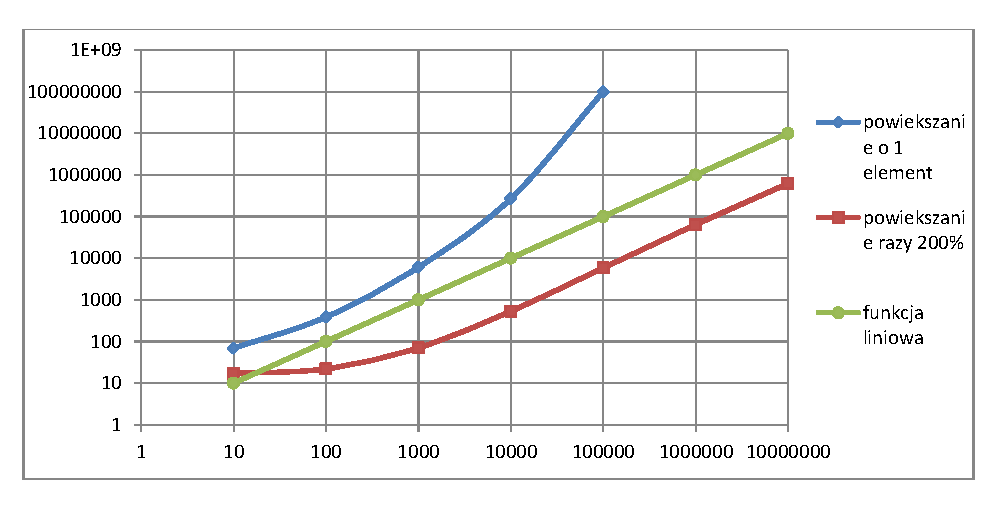
\includegraphics[width=14cm]{Wykres1.pdf}
	 	\caption{Wykres złożoności obliczeniowej.}
		 \end{figure}
		\section{Komentarz}
		Do utworzenia dokumentacji wykorzystano system Doxygen.
		Funkcja pomiaru czasu dla systemu Windows pobrana ze strony dr. J. Mierzwy. Program skompilowano w środowisku Code::Blocks. Do stworzonia wykresu posłużono się pakietem MS Excel, sprawozdanie napisano uzywając systemu \LaTeX.
\end{document}